\documentclass[addpoints,11pt]{exam}

\usepackage{alltt}
\usepackage[margin=1in]{geometry}   % set up margins
\usepackage[T1]{fontenc}
\usepackage[usenames,dvipsnames]{xcolor}
\usepackage{enumerate}              % fancy enumerate
\usepackage{amsmath}                % used for \eqref{} in this document
\usepackage{amsthm}
\theoremstyle{definition}
\newtheorem{exmp}{Example}[section]
\usepackage{verbatim}               % useful for \begin{comment} and \end{comment}
\usepackage{eurosym}                % used for euro symbol
\usepackage{caption} 
\usepackage{graphicx}
\graphicspath{{Figures/}}
\usepackage{subcaption}
\usepackage{color}
\usepackage{float}
\usepackage{amssymb}
\usepackage{sgamevar}
\usepackage{sgame}
\usepackage[colorlinks=true]{hyperref}
\hypersetup{colorlinks=true, citecolor=ForestGreen, linkcolor=BlueViolet, urlcolor=Magenta}



%Solutions or nah (blank next two lines out for no solutions, unblank #3)
%\printanswers
%\newcommand{\dd}[1]{\par {\textbf{\textcolor{red}{#1}}}}
\newcommand{\dd}[1]{}  


\setlength\parindent{0pt}
\unframedsolutions
\SolutionEmphasis{\color{red}}
\CorrectChoiceEmphasis{\color{red}}
\renewcommand{\choicelabel}{(\alph{choice})}
\newcommand{\blank}[0]{\underline{\hspace{3cm}}}
\pointformat{\bfseries[\thepoints]}
\pointpoints{pt}{pts}
\pointsinrightmargin

\begin{document}


\title{\textbf{Homework 3} \\ \dd{Solutions\\} \vspace{2 mm} {\large ECON 101}}
\author{Summer I 2016}
\date{}
\maketitle

\makebox[\textwidth]{Name:\enspace\hrulefill}
\\

\makebox[\textwidth]{ONYEN:\enspace\hrulefill}
\\

\makebox[\textwidth]{PID:\enspace\hrulefill}
\\

\begin{center}
	\fbox{\fbox{\parbox{5.5in}{\centering
			This homework is due on \textbf{May 26} by \textbf{1PM}. Show work for all questions that require it (including multiple choice questions), attaching extra sheets as necessary. Multiple choice answers should be bubbled in on a scantron. For the short answer section, write legibly and make sure to box final answers. The total number of points available on this assignment is \textbf{100}.}}}
\end{center}

\subsection*{Multiple Choice [2 pts each]}

\begin{questions}
	
			\question AJ opens a lemonade stand for two hours. He spends \$10 for ingredients and sells \$60 worth of lemonade. In those same two hours, he could have cleaned his neighbor's pool for \$40. AJ has an accounting profit of \blank and an economic profit of \blank.
			
			\begin{choices}
				\CorrectChoice \$50; \$10
				\choice \$90; \$50
				\choice \$10; \$50
				\choice \$50; \$90
			\end{choices}
			
			\begin{solution}
				Total revenue = \$60. Explicit costs = \$10. Implicit costs = \$40. Accounting profit = TR -- explicit costs = \$50. Economic profit = TR -- (explicit costs + implicit costs) = \$10.
			\end{solution}
			
			\question A firm is producing 100 units with an average total cost of \$25 and a marginal cost of \$15. If it were to increase production to 101 units, which of the following must occur?
			
			\begin{choices}
				\choice Marginal cost would decrease.
				\choice Marginal cost would increase.
				\CorrectChoice Average total cost would decrease.
				\choice Average total cost would increase.
			\end{choices}
			
			\begin{solution}
				If $MC < ATC$, then it must be that $ATC$ are decreasing.
			\end{solution}
			
			\question Bluth's Bananas currently employs 5 workers and produces 1,000 frozen bananas a day. In preparation for the busy summer season, the firm is debating whether they should hire 5 more workers. If they do, they project they could produce 1,500 frozen bananas a day. Given this, the marginal product of labor per worker from these additional workers would be
			
			\begin{choices}
				\choice 1,500.
				\choice 500.
				\choice 150.
				\CorrectChoice 100.
			\end{choices}
			
			\begin{solution}
				$MP_L = \frac{\Delta Q}{\Delta L} = \frac{(1,500 - 1,000)}{5} = 100.$
			\end{solution}
			
			\question Shell Tires has fixed costs of \$300,000 per year. Last year, it produced 10,000 tires with an average variable cost of \$80. What were the firm's average total costs for last year?
			
			\begin{choices}
				\choice \$80
				\choice \$90
				\choice \$100
				\CorrectChoice \$110
			\end{choices}
			
			\begin{solution}
				$ATC = TC/Q = (FC + VC)/Q = AFC + AVC = \$300,000/10,000 + \$80 = \$110$.
			\end{solution}
			
			\question Keystone Fireworks has fixed costs of \$100 and the marginal costs outlined in Table \ref{tab1}.
			
			\begin{table}[H]
				\caption{Marginal Costs for Keystone}
				\label{tab1}
				\centering
				%Change last column to "H" for solutions
				\begin{tabular}{ c|c H}      
					Quantity & Marginal Cost & \dd{Variable Costs}\\     
					\hline
					1 & \$2 & \dd{\$2} \\
					2 & \$4 & \dd{\$6} \\
					3 & \$6 & \dd{\$12}\\
					4 & \$8 & \dd{\$20}  \\
					5 & \$10 & \dd{\$30} \\
					6 & \$12 & \dd{\$42}\\
				\end{tabular}
			\end{table}
			
			What is the average variable cost of producing the fifth unit?
			
			\begin{choices}
				\choice \$2
				\CorrectChoice \$6
				\choice \$10
				\choice \$30
			\end{choices}
			
			\begin{solution}
				At Q=0, VC = \$0. At Q=1, MC = \$2 which means VC increased by \$2 when going from Q=0 to Q=1. So, at Q=1, VC = \$2. At Q=2, MC = \$4, so VC increased by \$4 when going from Q=1 to Q=2. Since VC=\$2 at Q=1, at Q=2 VC =\$6. Continuing this process until Q=5, we have that VC = \$30. AVC = VC/Q = \$30/5 = \$6.
			\end{solution}
			
			\question A firm currently produces 1,000 units of output with an average variable cost of \$5.10. The firm has fixed costs of \$5,000. If the firm were to produce 1,001 units, its total variable costs would be \$5,400. What is the marginal cost to the firm of producing 1,001 units?
			
			\begin{choices}
				\choice \$5,400
				\CorrectChoice \$300
				\choice \$5,100
				\choice \$400
			\end{choices}
			
			\dd{At 1,000 units, $VC = 1,000 \times 5.10 = \$5,100.$ $MC = \frac{\Delta VC}{\Delta Q} = \frac{(5,400 - 5,100)}{1} = \$300.$}
			
		\end{questions}
		
		\subsection*{Short Answer}
		
		\begin{questions}
			
			
			
			
			
			
			
			
			\question[4] Your roommate's food truck sells delicious burritos every Friday night. He tells you a story that as he closed up shop last weekend, an inebriated patron yelled at him to make him one for \$10.00. Your roommate had already sold 200 burritos that night, but usually has to sell them for \$4.00 due to market conditions. He tells you that he obviously sold him the burrito for \$10.00. If he faces the cost schedule detailed in Table \ref{tab5}, was this the right decision? Explain why or why not. 
			
			
			\begin{table}[H]
				\caption{Burrito Costs}
				\centering
				\begin{tabular}{ c|c}        
					
					Quantity  & ATC \\
					\hline
					199 & \$1.99 \\
					200 & \$2.00 \\
					201 & \$2.05 \\
				\end{tabular}
				\label{tab5}
			\end{table}
			
			\begin{solution}
				Your roommate should sell the burrito as long as $MR \ge MC$. $MR = \$4.$ At Q=200, $TC = \$2.00 \times 200 = \$400$ and at Q=201 $TC = \$2.05 \times 201 = \$412.05.$ $MC = 412.05 - 400 = \$12.05$. Your friend should not have the sold burrito for \$10, as he would actually decrease his profit for the day by \$2.05.
			\end{solution}
			
			
			\question What topics or questions gave you the most trouble on this homework assignment or the class material it encompassed? 
			
			
			\question If a profit-maximizing competitive firm is producing a quantity at which marginal cost is between average variable cost and average total cost, it will
			
			\begin{choices}
				\CorrectChoice keep producing in the short run, but exit the market in the long run.
				\choice shut down in the short run, but return to production in the long run. 
				\choice shut down in the short run and exit in the long run.
				\choice keep producing in both the short run and the long run.
			\end{choices}
			
			\begin{solution}
				A competitive firm produces where $P = MC$. For prices where $AVC < P < ATC$, the firm produces in the short-run, but will shut down in the long-run.
			\end{solution}
	
		
		\question Profit for a firm in a perfectly competitive market is positive whenever
		
		\begin{choices}
			\choice $P < ATC$.
			\choice  $P < MC$.
			\choice $P > MC$.
			\CorrectChoice $P >ATC$.
		\end{choices}
		
		\begin{solution}
			$\Pi = TR - TC  = (P - ATC)\cdot Q \Rightarrow \Pi >0 \iff P > ATC$.
		\end{solution}
	
		\question Consultants hired by Sunnyside Eggs find that the firm has total fixed costs of \$50,000, total variable costs of \$25,000, and total revenues of \$40,000. Given this, in the short run the firm should \blank and make \blank profit.
		
		\begin{choices}
			\choice shut down; negative
			\choice shut down; zero
			\CorrectChoice stay open; negative
			\choice stay open; positive
		\end{choices}
	
			
		\begin{solution}
			Short-run decision: Shut down if $TR<VC$, operate if $TR>VC$. Firm should operate in the short run. $\Pi = TR - TC = \$40,000 - (50,000 + 25,000) = -\$35,000.$
		\end{solution}
		
\uplevel{For questions \ref{blah1} and \ref{blah2}, refer to Table \ref{tab2}.}
				\begin{table}[H]
							\centering
							\caption{Competitive Firm}
							\label{tab2}
							%Change to H's for HW
							\begin{tabular}{ c|c|c}        
								
								Quantity & Total Revenue & Total Cost  \\
								\hline
								0 & \$0  & \$30 \\
								1 & \$80 & \$50 \\
								2 & \$160 & \$80 \\
								3 & \$240 & \$120 \\
								4 & \$320 & \$170  \\
								5 & \$400 & \$230 \\
								6 & \$480 & \$300  \\
								7 & \$560 & \$380 \\
								8 & \$640 & \$470   \\
							\end{tabular}
						\end{table} 

			
			\question \label{blah1} What is the marginal cost at the profit maximizing quantity?
			\begin{choices}
				\choice \$50
				\CorrectChoice \$80
				\choice \$230
				\choice \$300
			\end{choices}
			
			\begin{solution}
				Maximize profit at $Q$ where $MR = MC.$
			\end{solution}
			
			\question \label{blah2} What is the average fixed cost at the profit maximizing quantity?
			
			\begin{choices}
				\choice \$54.30
				\CorrectChoice \$4.28
				\choice \$50
				\choice \$80
			\end{choices}
			
			\begin{solution}
				$Q^* = 7$ (where $MR = MC).$ $FC = \$30$ (total cost at $Q=0$). $AFC = FC/Q = \$30/7 = \$4.28$.
			\end{solution}
			
			
			\question Natalie the baker wants to establish a pie factory in a competitive market. The cost of leasing the factory is \$800 a day. The profit maximizing quantity of pies is 1,000 a day, each pie sells for \$3, and has a variable cost of only \$1.50. Which of the following is true?
			
			\begin{choices}
				\CorrectChoice Natalie should enter the industry.
				\choice Natalie should not enter the industry.
				\choice Natalie would enjoy profits of \$3,000 a day.
				\choice Both (a) and (c) are true.
			\end{choices}
			
			\begin{solution}
				Enter market if $TR \ge TC \iff P \ge ATC$. $TR = \$3\cdot 1,000 = \$3,000$ and $TC = \$800 + \$1.50\cdot 1,000 = \$2,300$. Thus, Natalie should enter the market and will make a profit of $\$3,000 - \$2,300 = \$700/\text{day}.$
			\end{solution}
			
			\question In order to maximize profit, a firm in a perfectly competitive market will produce at the quantity where
			
			\begin{choices}
				\CorrectChoice $AR = MC$.
				\choice $P = ATC$.
				\choice $P = AVC$.
				\choice $MR = ATC$.
			\end{choices}

	\begin{solution}
		Always produce where $MR = MC$. For competitive firms, $MR = P = AR$.
	\end{solution}
	
\newpage

	\question Al's Burgers is a firm in a competitive market and faces the cost structure shown in Figure \ref{MC28}.
				
				\begin{figure}[htp]
					\centering
					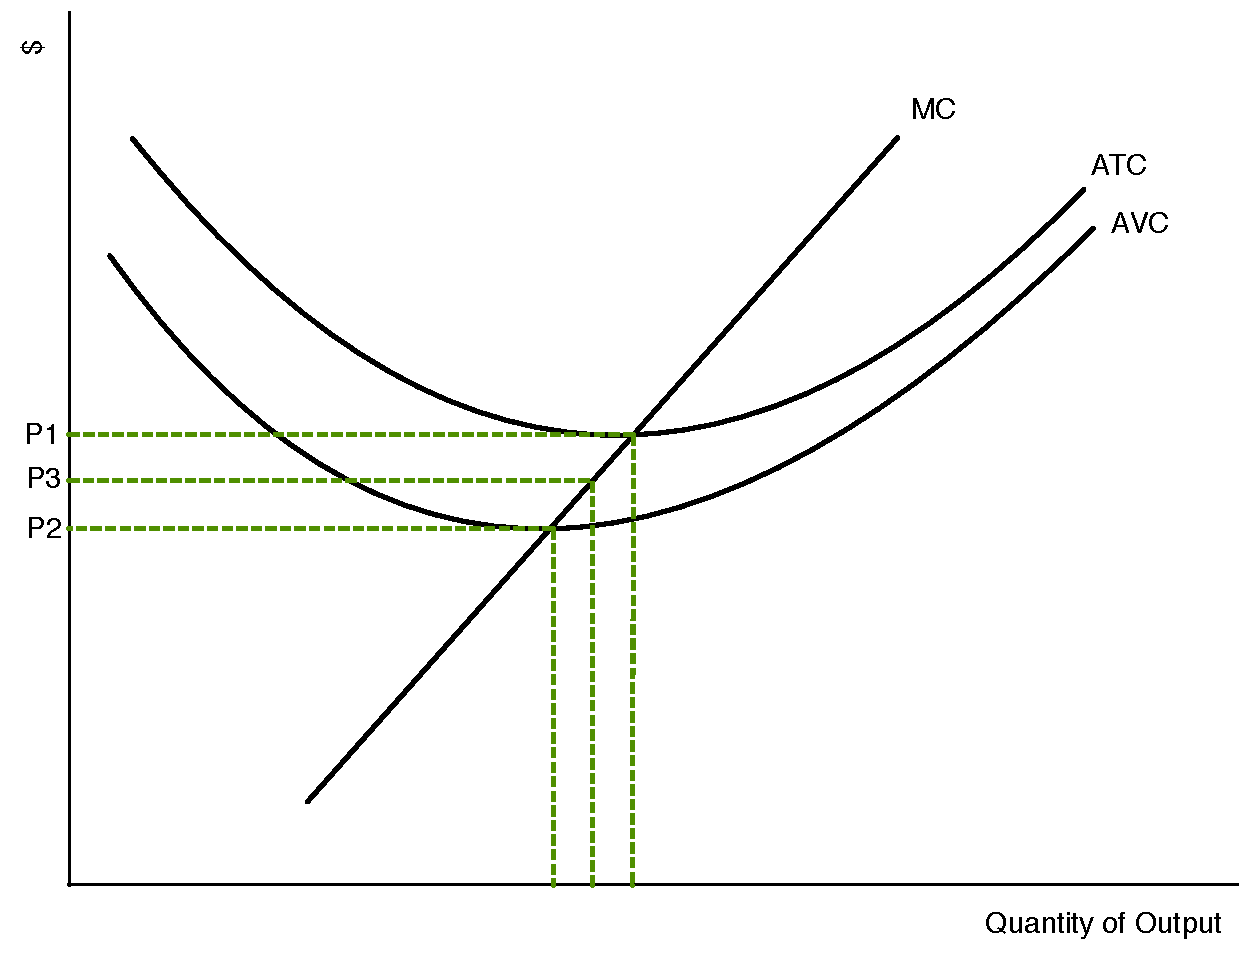
\includegraphics[scale=.45]{Exam1_MC27.pdf}
					\caption{Al's Burgers}
					\label{MC28}
				\end{figure}
				
				The firm decides to operate in the short run, but incurs economic losses. Thus, the market price must be 
				
				\begin{choices}
					\choice less than P2.
					\choice greater than P2 but less than P3.
					\choice greater than P3 but less than P1.
					\CorrectChoice greater than P2 but less than P1.
					\choice greater than P1.
				\end{choices}
				
			\begin{solution}
				Operate in SR along $MC$ curve above $AVC$. If operating at a loss, $P<ATC$ and so price must be $P2 < P < P1$.
			\end{solution}
				
				
	\question Suppose the market for corn is perfectly competitive. Which of the following represents the long-run relationship between the price, marginal cost, and average total cost at the profit-maximizing quantity?
	
	\begin{choices}
		\choice $P > MC = ATC$
		\choice $P = MC > ATC$ 
		\CorrectChoice $P = MC = ATC$
		\choice $P > MC > ATC$
	\end{choices}
	
	\begin{solution}
		Firms in PC produce where $P = MC$. In the long run, firms in PC make zero economic profit so $P=ATC$.
	\end{solution}
			

			\question Assuming the same cost structure, a competitive market produces \blank output at \blank prices than a monopoly market.
			
			\begin{choices}
				\choice less; lower
				\CorrectChoice more; lower
				\choice less; higher
				\choice more; higher
			\end{choices}
			
			\begin{solution}
				Monopolies charge a mark-up over the marginal cost and produce less than a competitive market.
			\end{solution}

\newpage

		
\uplevel{Refer to Table \ref{tab3} for questions \ref{blah3} and \ref{blah4}.} 

		\begin{table}[h!]
			\caption{Monopolist Environment}
			\label{tab3}
			\centering
			\begin{tabular}{  c|c|c}    
				Price & Quantity Demanded & Total Cost \\    
				\hline
				\$170 & 0 & \$100 \\
				\$160 & 1 & \$140 \\
				\$150 & 2 & \$184 \\
				\$140 & 3 & \$230 \\
				\$130 & 4 & \$280 \\
				\$120 & 5 & \$335 \\
				\$110 & 6 & \$395 \\
				\$100 & 7 & \$475 \\ 
				\$90 & 8 & \$565 \\
			\end{tabular}
		\end{table}

			
			\question \label{blah3} What is the marginal cost of the 6$^{th}$ shirt?
			
			\begin{choices}
				\choice \$44
				\choice  \$46
				\choice  \$55
				\CorrectChoice \$60
			\end{choices}
			
			\begin{solution}
				$MC = \Delta TC/ \Delta Q$. At $Q=6$, $MC = 395 - 335 = \$60.$
			\end{solution}
			

			\question \label{blah4} What is total profit at the profit-maximizing quantity?
			
			\begin{choices}
				\choice \$100
				\choice \$245
				\CorrectChoice \$265
				\choice \$395
			\end{choices}
			
			\begin{solution}
				Maximize profit where $MC = MR$. $MR = \Delta TR/\Delta Q$, so need to find $TR = P\times Q$ at each price first, then find $MR$. $MR$ = $MC$ = \$60 at $Q=6$, so $Q^* =6$ and $\Pi = \$660 - 395 = \$265$.
			\end{solution}


\uplevel{Use Figure \ref{MC10}, which represents the environment faced by a monopoly, for questions \ref{blah5} and \ref{blah6}.}

\begin{figure}[h!]
	\centering
	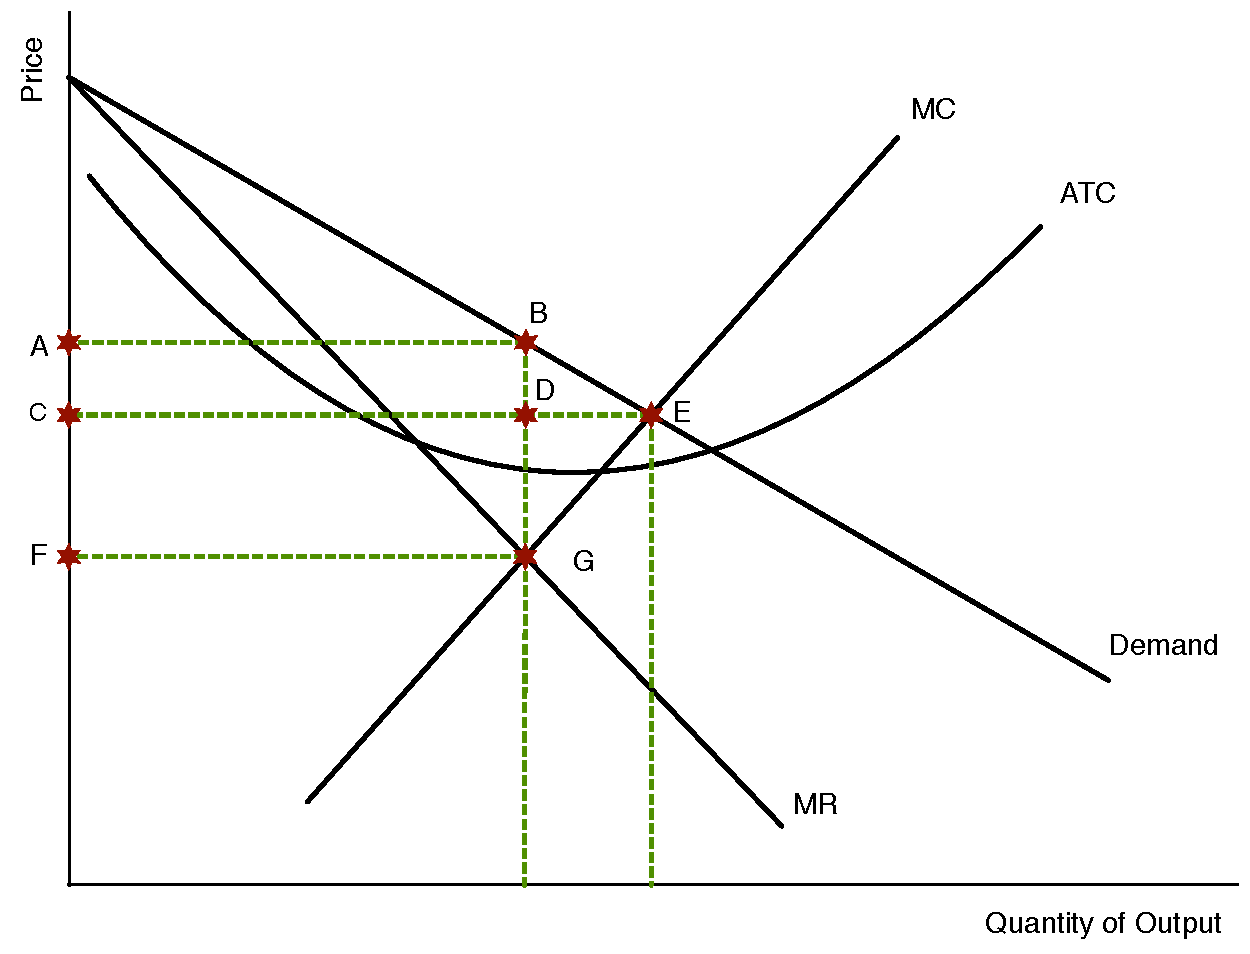
\includegraphics[scale=.4]{Exam2_MC10.pdf}
	\caption{Monopolist Environment}
	\label{MC10}
\end{figure}

\newpage


	\question \label{blah5} Which of the following represents the lost trade that is responsible for the deadweight loss?
	
	\begin{choices}
		\choice Distance ab
		\choice Distance ce
		\CorrectChoice Distance de
		\choice Distance cd
	\end{choices}
	
	\begin{solution}
		Optimal quantity where $MC$ = Demand. Monopolist produces where $MR = MC$. Lost trades between distance de.
	\end{solution}
	
	\question \label{blah6} Which of the following areas represents the deadweight loss due to monopoly pricing?
	
	\begin{choices}
		\CorrectChoice Triangle bge
		\choice Triangle bde
		\choice Rectangle acdb
		\choice Rectangle cfgd
	\end{choices}
	
	\begin{solution}
		DWL comes from those trades that are not taking place where demand is above $MC$.
	\end{solution}
	
	
\question Consider Figure \ref{MC35}, which shows the cost structure of a monopolist.


\begin{figure}[h!]
	\centering
	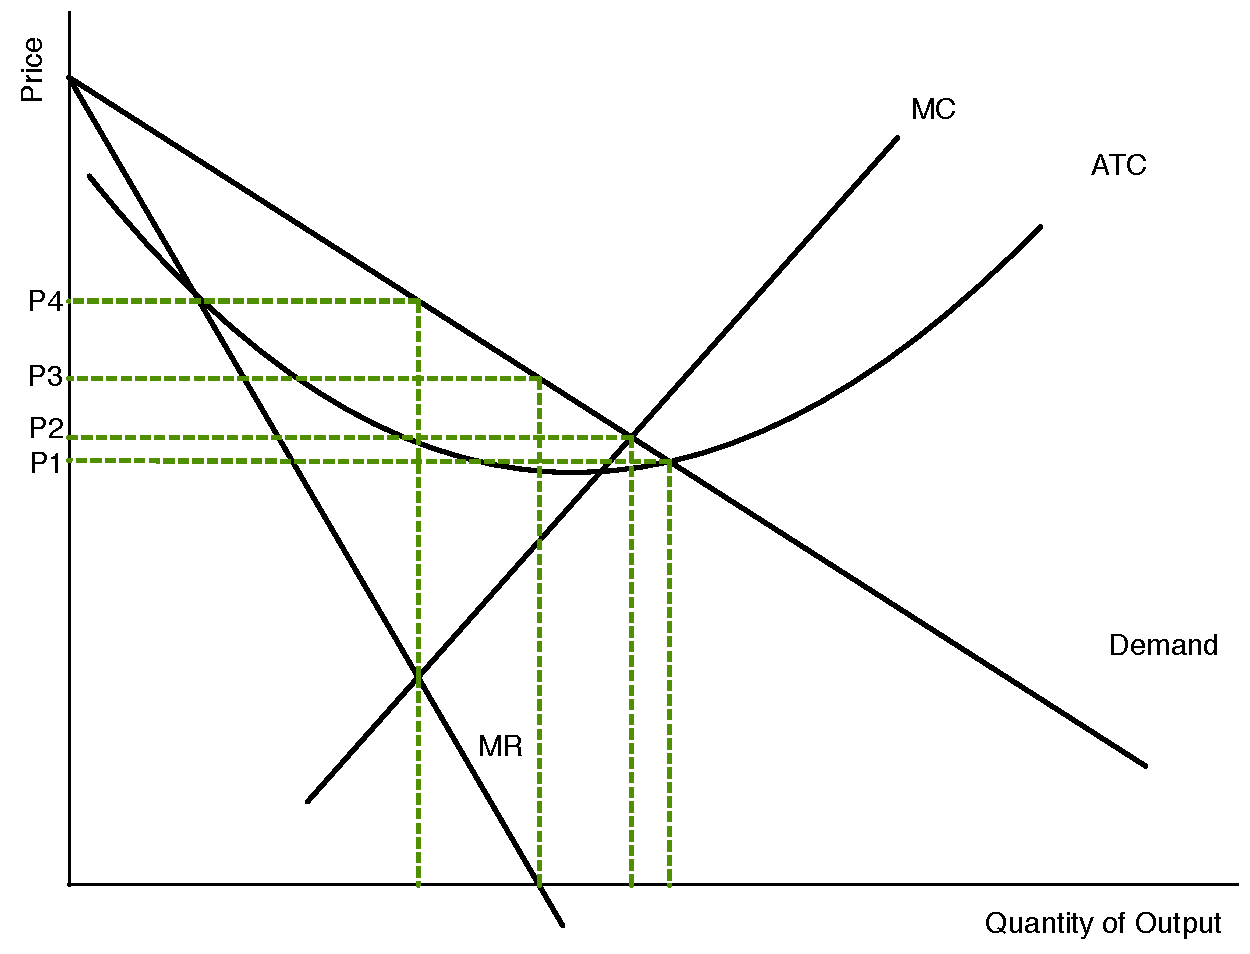
\includegraphics[scale=.40]{Final_MC35.pdf}
	\caption{Monopolist Environment}
	\label{MC35}
\end{figure}

If the firm wishes to maximize total revenue, it should charge price \underline{\hspace{3cm}}, while the price it should charge to maximize output while not making losses is \underline{\hspace{3cm}}.

\begin{choices}
	\choice P4; P2
	\CorrectChoice P3; P1
	\choice P2; P4
	\choice P3; P2
	\choice None of the above
\end{choices}

\begin{solution}
	Maximize $TR$ where at $Q$ where $MR = 0$. Trace up to demand curve to find price ($P3$). Losses occur when $P<ATC$. Lower price until $P=ATC$ to maximize output while not making losses. $P = P1$.
\end{solution}

\newpage

	\question A profit-maximizing monopolist will produce the level of output at which
	
	\begin{choices}
		\choice average revenue is equal to average total cost.
		\choice price is equal to marginal cost.
		\CorrectChoice marginal revenue is equal to marginal cost.
		\choice total revenue is equal to opportunity cost.
	\end{choices}
	
	\begin{solution}
		Any firm should produce where $MR = MC$ in order to maximize profits. This holds true in any type of market structure. (b) is only true for firms in a perfectly competitive market.
	\end{solution}
	
	
	\question If economies of scale exist, and government regulators force the monopolist to set price equal to marginal cost,
	
	\begin{choices}
		\choice the monopolist will still earn a profit, just smaller than with no regulation.
		\choice there will be no incentive to innovate.
		\choice the market will be less efficient than if regulators set prices equal to average total cost.
		\CorrectChoice the monopolist will be taking a loss.
	\end{choices}
	
	\begin{solution}
		For monopolies with economies of scale, $MC < ATC$. If the government forces the monopolist to charge $P=MC$ (this is the point where the demand and MC curve meet), then $P<ATC$ and $\Pi <0$.
	\end{solution}


		
		\question Which of the following conditions does NOT describe a firm in a monopolistically competitive market?
		
		\begin{choices}
			\choice It makes a product different from its competitors.
			\CorrectChoice It takes its price as given by market conditions.
			\choice It maximizes profit both in the short run and in the long run.
			\choice It has the freedom to enter or exit in the long run.
		\end{choices}
		
		\begin{solution}
			See class notes.
		\end{solution}
		
	\question Firms in monopolistically competitive markets are similar to monopolies in that they both \blank and are similar to firms in perfectly competitive markets in that they both \blank.
			
			\begin{choices}
				\choice make positive profits in the short and long run; are price takers
				\choice charge a price above the marginal cost; produce at the efficient scale in the long run
				\CorrectChoice are price makers; make zero economic profit in the long run
				\choice are in markets with barriers to entry; produce at the efficient quantity
			\end{choices}
			
		\begin{solution}
			See class notes.
		\end{solution}
			
	\question A monopolistically competitive firm will decrease its production if
		
		\begin{choices}
			\choice marginal revenue is less than average total cost.
			\choice price is less than marginal cost.
			\CorrectChoice marginal revenue is less than marginal cost.
			\choice price is less than average total cost.
		\end{choices}
		
		\begin{solution}
			See class notes.
		\end{solution}
		
		\newpage
			
			
		\question For a firm in a monopolistically competitive market, which of the following accurately describes the relationship between the price, average total cost, and marginal cost in the short run given that the firm is making a negative profit?
		
		\begin{choices}
			\choice $ATC = P = MC$
			\choice $ATC > P = MC$
			\choice $ATC = P > MC$
			\CorrectChoice $ATC > P > MC$
		\end{choices}
		
		\begin{solution}
			Firms in monopolistically competitive markets charge a mark-up over $MC$, so $P>MC$. If making a loss, $P<ATC$.
		\end{solution}
			
			
		\question For a firm in a monopolistically competitive market, which of the following accurately describes the relationship between the price, average total cost, and marginal cost in the long run?
		
		\begin{choices}
			\choice $P = ATC = MC$
			\choice $P > ATC = MC$
			\CorrectChoice $P = ATC > MC$
			\choice $P > ATC > MC$
		\end{choices}
		
		\begin{solution}
			In long run, firms in monopolistically competitive markets make zero economic profit so $P=ATC$. Still charge mark-up over $MC$ so $P>MC$.
		\end{solution}
		
		\question Consider the environment faced by Sparkle, one of the many toothpaste brands in the market for toothpaste, shown in Figure \ref{fig1}.
		
		\begin{figure}[ht!]
			\centering
			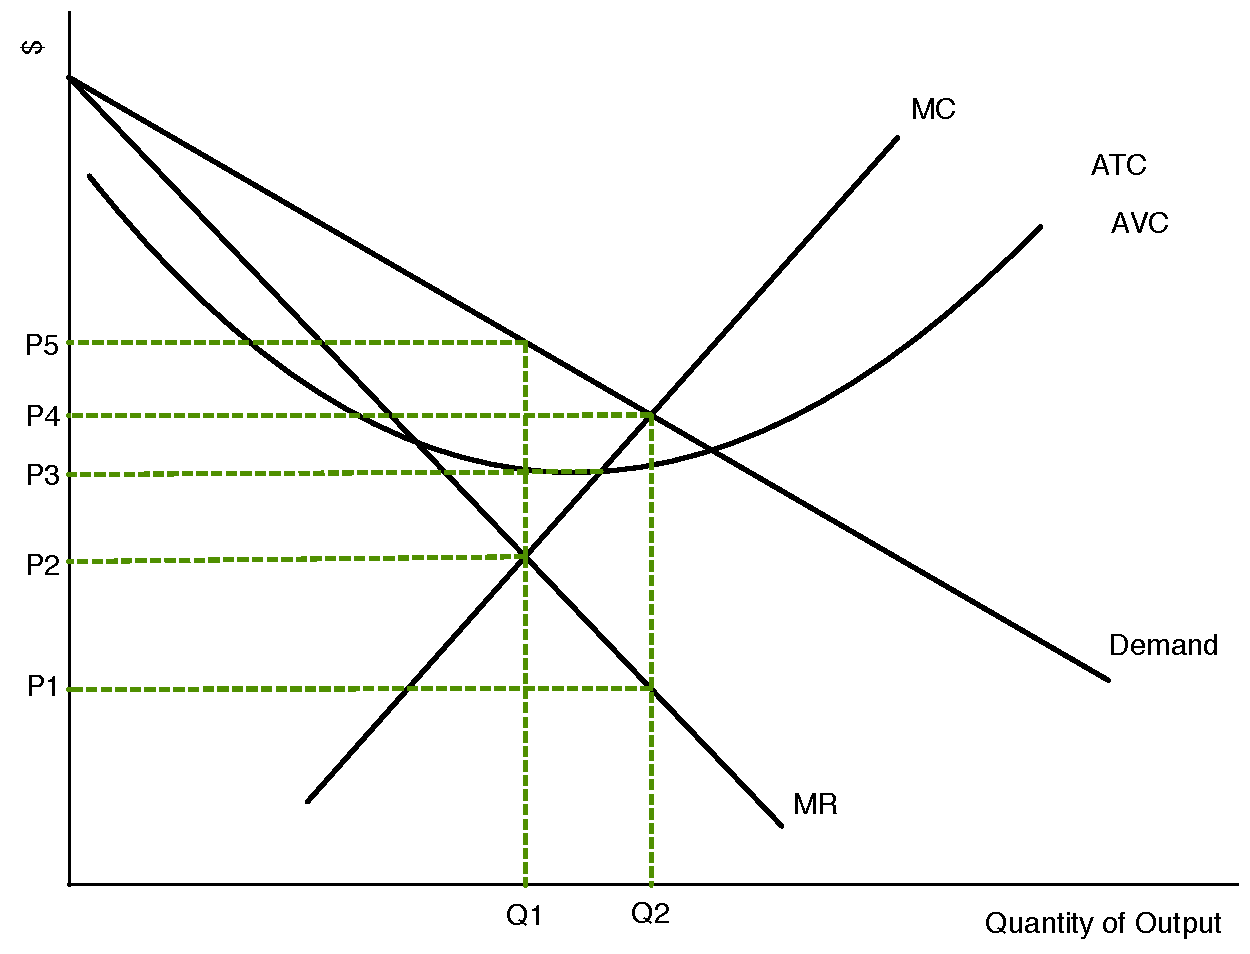
\includegraphics[scale=.40]{hw5_plot1.pdf}
			\caption{Environment for Sparkle}
			\label{fig1}
		\end{figure}
		
		The quantity produced by the firm is \underline{\hspace{3cm}} and it charges a markup of \\ \underline{\hspace{3cm}}.
		
		\begin{choices}
			\choice $Q2; P4-P3$
			\choice $Q2; P4-P1$
			\choice $Q1; P3-P2$
			\CorrectChoice $Q1; P5-P2$
		\end{choices}
		
		\begin{solution}
			Produce at $Q$ where $MR = MC$ ($Q1$). Price is point on demand curve at $Q1$ which is $P5$. Mark-up over the marginal cost = $P5 - P2$
		\end{solution}
		
\newpage
		
		\question If an oligopolistic industry organizes itself as a cooperative cartel, it will produce a quantity of output that is \blank the competitive level and \blank the monopoly level.
		
		\begin{choices}
			\choice less than; more than
			\choice more than; less than
			\CorrectChoice less than; equal to
			\choice equal to; more than
		\end{choices}
		
		\begin{solution}
			When acting as a cartel, firms act like a monopolist. The monopolist quantity is less than the competitive quantity.
		\end{solution}

		\question If an oligopoly does not cooperate and each firm chooses its own quantity, the industry will produce a quantity of output that is \blank the competitive level and \blank the monopoly level.
		
		\begin{choices}
			\CorrectChoice less than; more than
			\choice more than; less than
			\choice less than; equal to
			\choice equal to; more than
		\end{choices}
		
		\begin{solution}
			Self-interest drives firms to break cartel agreement and produce more, but will still produce less than in perfect competition.
		\end{solution}

	
\uplevel{For questions \ref{blah7} and \ref{blah8}, consider the simultaneous move game below.}
	
	\renewcommand{\gamestretch}{1.5}
	\sgcolsep=25pt
	\begin{figure}[htb]\hspace*{\fill}%
		\begin{game}{2}{2}[Mexico][United States] 
			&  Low tariffs & High Tariffs \\
			Low tariffs & \$25M, \$25M & \$10M, \$30M \\
			High tariffs & \$30M, \$10M & \$20M, \$20M \\
		\end{game} 
		\hspace*{\fill}%
	\end{figure}
	

		\question \label{blah7}The dominant strategy for Mexico is \blank and the dominant strategy for the US is \blank.
		
		\begin{choices}
			\choice low tariffs; low tariffs
			\choice high tariffs; low tariffs
			\choice low tariffs; high tariffs
			\CorrectChoice high tariffs; high tariffs
		\end{choices}
		
		\begin{solution}
			If US plays low tariffs, Mexico better of choosing high tariffs (30>25). If US plays high tariffs, Mexico still better off playing high tariffs (20>10). HT is dominant strategy for Mexico. Same for US.
		\end{solution}
		
		\item \label{blah8} Thus, the Nash Equilibrium is where the United States plays \blank and Mexico plays \blank.
		
		\begin{choices}
			\choice low tariffs; low tariffs
			\choice high tariffs; low tariffs
			\choice low tariffs; high tariffs
			\CorrectChoice high tariffs; high tariffs
		\end{choices}
		
		\begin{solution}
			Neither country can do better given the other country's strategy at (HT, HT).
		\end{solution}
		
		\newpage
		
		\question Intel and AMD each decide to either invest heavily in R\&D (``High R\&D'') or to not (``Low R\&D''). Their decisions affect both their profits and those of the other company. Assume that there is perfect information so that each knows the payoffs of the other given the strategies chosen by each. Their profits are summarized in the game table below, where the first number in each block is AMD's profit and the second number is Intel's profit.
		
		\renewcommand{\gamestretch}{1.5}
		\sgcolsep=25pt
		\begin{figure}[htb]\hspace*{\fill}%
			\begin{game}{2}{2}[AMD][Intel] 
				&  High R\&D & Low R\&D \\
				High R\&D & \$15,000, \$20,000 & \$18,000, \$15,000 \\
				Low R\&D & \$16,000, \$18,000 & \$16,000, \$15,000\\
			\end{game} 
			\hspace*{\fill}%
		\end{figure}
		
		If this game was played once and Intel and AMD are both rational, what would be the outcome?
		
		\begin{choices}
			\CorrectChoice Intel would invest heavily in R\&D and AMD would not.
			\choice Both Intel and AMD would invest heavily in R\&D.
			\choice AMD would invest heavily in R\&D and Intel would not.
			\choice Both Intel and AMD would choose to not invest heavily in R\&D.
		\end{choices}
		
		\begin{solution}
			AMD has no dominant strategy, but Intel has dominant strategy of high R\&D. Since AMD knows the payoffs, they know Intel has dominant strategy and that Intel will choose high R\&D. AMD's best response to this is Low R\&D. Nash eq: (low, high).
		\end{solution}
		
		\question Consider the simultaneous move game between Righty and Lefty shown below, where the first number in each block is the payoff to Lefty and the second is the payoff to Righty.
		
		\renewcommand{\gamestretch}{1.5}
		\sgcolsep=25pt
		\begin{figure}[htb]\hspace*{\fill}%
			\begin{game}{2}{2}[Lefty][Righty] 
				&  Swerve & Straight \\
				Swerve & 2, 2 & $x$, 4 \\
				Straight & 1, $y$ & 2, 3 \\
			\end{game} 
			\hspace*{\fill}%
		\end{figure}
		
		If this particular game has \textbf{no} Nash equilibrium, then possible values of $x$ and $y$ are
		
		\begin{choices}
			\choice $x=1$ and $y=2$.
			\CorrectChoice $x=1$ and $y=4$.
			\choice $x=3$ and $y=2$.
			\choice $x=3$ and $y=4$.
		\end{choices}
		
		\begin{solution}
			Lefty: If Righty chooses swerve, Lefty will choose swerve (2>1). Needs to pick Straight if Righty chooses Straight in order to not have dominant strategy $\Rightarrow x < 2.$ \\
			Righty: If Lefty chooses Swerve, Righty will choose straight (4>2). Needs to pick Swerve if Lefty chooses Straight in order to not have dominant strategy $\Rightarrow y>3.$
		\end{solution}
		


	\question Consider the simultaneous move game between Jim and Bob shown below, where the first number in each block is the payoff to Bob and the second is the payoff to Jim.
	
	\renewcommand{\gamestretch}{1.5}
	\sgcolsep=25pt
	\begin{figure}[htb]\hspace*{\fill}%
		\begin{game}{2}{2}[Bob][Jim] 
			&  Left & Right \\
			Top & 2, 4 & $x$, 2 \\
			Bottom & 1, $y$ & 2, 3 \\
		\end{game} 
		\hspace*{\fill}%
	\end{figure}
	
\newpage
	
	If ``Top'' is the dominant strategy for Bob and ``Left'' is the 	dominant strategy for Jim, then possible values of $x$ and $y$ are
	
	
	\begin{choices}
		\choice $x=1$ and $y=2$.
		\choice $x=1$ and $y=4$.
		\choice $x=3$ and $y=2$.
		\CorrectChoice $x=3$ and $y=4$.
	\end{choices}
	
	\begin{solution}
		Bob: Needs to choose Top when Jim chooses Right $\Rightarrow x>2$.\\
		Jim: Needs to choose Left when Bob chooses Bottom $\Rightarrow y>3$.
	\end{solution}
	
\end{questions}

\subsection*{Short Answer}

\begin{questions}
	
	\question Natalie's Ball Bearings, Inc. faces the following costs of production outlined in Table \ref{tab4}.
	
	\begin{table}[h]
		\centering
		\caption{Cost of Ball Bearings}
		\label{tab4}
		\begin{tabular}{  c|c|c}        
			
			Quantity (in cases) & Total Fixed Costs & Total Variable Costs \\
			\hline
			0 & \$100  &  \\
			1 &  & \$50 \\
			2 &  & \$70 \\
			3 &  & \$90  \\
			4 &  & \$140 \\
			5 &  & \$200 \\
			6 &  & \$360  \\
		\end{tabular}
	\end{table} 
	
	\begin{parts}
		\part[4] Suppose the market for ball bearings is perfectly competitive and the price of a case is \$50. The CEO sees that he can't make a profit, and so decides to shut down operations. What is the firm's profit (or loss) as a result of this decision? Do you agree with the CEO's decision? Why or why not? 
		
		\begin{solution}
			If firm shuts down, $TR$ = 0, $VC$ = 0, and $FC$ = \$100 so $\Pi = -\$100$. \\
		 To find optimal quantity, use variable cost column to compute $MC$. $MC$ = \$50 at $Q=1$ and $Q=4$. At $Q=1$, $\Pi = \$50 \times 1 - \$150 = -\$100$. At $Q=4$, $\Pi = \$50 \times 4 - \$240 = -\$40$. Don't agree since $TR > VC$ at $Q=4$, the firm should produce in the SR even if it is making losses since it would lose more by shutting down.
		\end{solution}
		
		\part[4] If instead the CEO decided to produce 1 case of ball bearings, what would be the firm's profit (or loss)? Is this the best decision? Why? 
		
		\begin{solution}
			See (a). Always produce on part of $MC$ curve past its minimum. $MC$ decreases from $Q=1$ to $Q=2$, so $Q=1$ cannot be optimal quantity.
		\end{solution}
	\end{parts}
	
		
		\question Sleek Sneakers Co. is one of the many firms in the market for shoes, where each company sells differentiated products.
		
		\begin{parts}
			\part[2] Assume that Sleek is currently earning short-run profit. On a clearly labeled diagram, show the company's profit maximizing output and price, as well as the area representing profit. 
			
			\begin{solution}
				See class notes. If profit is positive, $P>ATC$ at the profit maximizing quantity, which is given by where $MR=MC$.
			\end{solution}
			
			\part[2] What happens to Sleek's price, output, and profit in the long run? Show this in a new diagram. 
			
			\begin{solution}
				In the long run, other firms enter the market. Demand for Sleek shoes decreases and becomes more elastic. In LR, demand and ATC are tangent at the profit maximizing quantity since firms make zero economic profit. Price, output, and profit decreases.
			\end{solution}
			
			\part[2] On your diagram for the firm in the long run, show the consumer surplus derived from the purchase of Sleek shoes and the deadweight loss relative to the efficient level of output. 
			
			\begin{solution}
				See class notes. CS is area above the price and below the demand curve. DWL comes from lost trades where demand is above $MC$.
			\end{solution}
			
			\part[2] If the government forced Sleek to produce the efficient level of output, what would happen to the firm? 
			
			\begin{solution}
				Efficient level of output is where $P=MC$, or where demand and $MC$ intersect. But at this price, $P<ATC$ and so the firm would be making a loss.
			\end{solution}
			
		\end{parts}
		
		\newpage
		
		\question Jack and Jill are the only lemonade providers in Jurassic World. They face the environment outlined in Table \ref{MC21}. 
		
			\begin{table}[h!]
				\caption{Demand Schedule and Costs Lemonade}
				\centering
				\begin{tabular}{c|c|c}
					Price & Quantity Demanded & Average Total Cost \\
					\hline
					\$1.10 & 300 & \$.30\\
					\$1.00 & 400 & \$.30\\
					\$.90 & 500 & \$.30\\
					\$.80 & 600 & \$.30 \\
					\$.70 & 700 & \$.30 \\
					\$.60 & 800 & \$.30 \\
				\end{tabular} 
				\label{MC21}
			\end{table}
			
			
		\begin{parts}
			
			\part[2] The two friends currently have an agreement where they produce 600 drinks in total and split production evenly. What will be the profit realized by each individual? 
			
			\begin{solution}
				To sell 600 drinks, they will charge price of \$.80 and realize total profit of $\Pi = (.80 - .30)\times 600 = \$300$. Since they split production, profit of each will be \$150.
			\end{solution}
			
			\part[2] If Jack were to break this agreement and increase his lemonade stand's production by 100 drinks, while Jill stuck to the original agreement, what will be the profit realized by each?
			
			\begin{solution}
				With quantity demanded of 700, price will decrease to \$.70. Jack will realize profit of $\Pi = (.70 - .30) \times 400 = \$160$, while Jill will only realize profit of $\Pi = (.70 - .30) \times 300 = \$120$.
			\end{solution}
			
			\part[4] What will be the profit realized by each if both choose to increase production by 100 units? 
			
			\begin{solution}
				New price will be \$.60 since quantity demanded is 800. Profit for each is $\Pi = (.60 - .30) \times 400 = \$120$.
			\end{solution}
			
		
		\end{parts}


		
		\question Consider the three person simultaneous move game below. Each person can decide to either work or shirk. Alice chooses the row, Bob chooses the column, and Curt chooses the matrix. For example, if Alice decides to work, Bob decides to shirk, and Curt decides to work, the payoffs are given by the top row of the right column of the top matrix. Alice would get a payoff of $-1/2$, Bob would get a payoff of $3/2$, and Curt would get a payoff of $1$.
	
		
		\begin{center} Curt: Work \end{center}
		\renewcommand{\gamestretch}{1.5}
		\sgcolsep=25pt
		\begin{figure}[h!]\hspace*{\fill}%
			\begin{game}{2}{2}[Alice][Bob] 
				&  Work & Shirk \\
				Work & 1, 1, 1 & $-1/2$, $3/2$, 1 \\
				Shirk & $3/2$, 1, $-1/2$ & 0, $3/2$, $-1/2$ \\
			\end{game} 
			\hspace*{\fill}%
		\end{figure}
		
		\begin{center} Curt: Shirk \end{center}
		\renewcommand{\gamestretch}{1.5}
		\sgcolsep=25pt
		\begin{figure}[htb]\hspace*{\fill}%
			\begin{game}{2}{2}[Alice][Bob] 
				&  Work & Shirk \\
				Work & 1, $-1/2$, 3/2 & $-1/2$, 0, 3/2 \\
				Shirk & $3/2$, $-1/2$, 0 & 0, 0, 0 \\
			\end{game} 
			\hspace*{\fill}%
		\end{figure}
		
\newpage
		
		\begin{parts}
			\part[2] Does Alice have a dominant strategy? If so, what is it? 
			
			\begin{solution}Top matrix: Curt chooses work. If Bob works, Alice better off shirking (3/2>1). If Bob shirks, Alice is better off shirking (0>--1/2). \\
				Bottom matrix: Curt chooses shirk. If Bob works, Alice is better off shirking (3/2>1). If Bob shirks, Alice is better off shirking (0>--1/2). \\
				Since Alice is better off shirking regardless of the other players' strategies, her dominant strategy is to shirk.
			\end{solution}
			
			\part[2] Does Bob have a dominant strategy? If so, what is it?
			
			\begin{solution}
				Similar analysis to (a). Dominant strategy is to shirk.
			\end{solution}
			
			\part[2] Does Curt have a dominant strategy? If so, what is it? 
			\begin{solution}
				A little trickier, as you have to compare entries across the matrices. For example, if Alice and Bob both work, Curt's payoffs are either 1 if he works (3rd entry of top left corner of top matrix) or 3/2 (3rd entry of top left corner of bottom matrix). Continuing this way for each Alice and Bob strategy combination, Curt's dominant strategy is also to shirk.
			\end{solution}
			
			\part[2] If there is one, what is the Nash equilibrium in this game? 
			\begin{solution}
				Nash eq. is (shirk, shirk, shirk). Payoff are given by bottom right corner of the bottom matrix.
			\end{solution}
		\end{parts}
		
	
	\question What topics or questions gave you the most trouble on this homework assignment or the class material it encompassed? 
		
\end{questions}


\end{document}